\section{Orphan section formerly the improvement section}

[not sure what to do with the following material? is it part of the critique section or the conclusion?]

\begin{figure}[!ht]
  \centering
    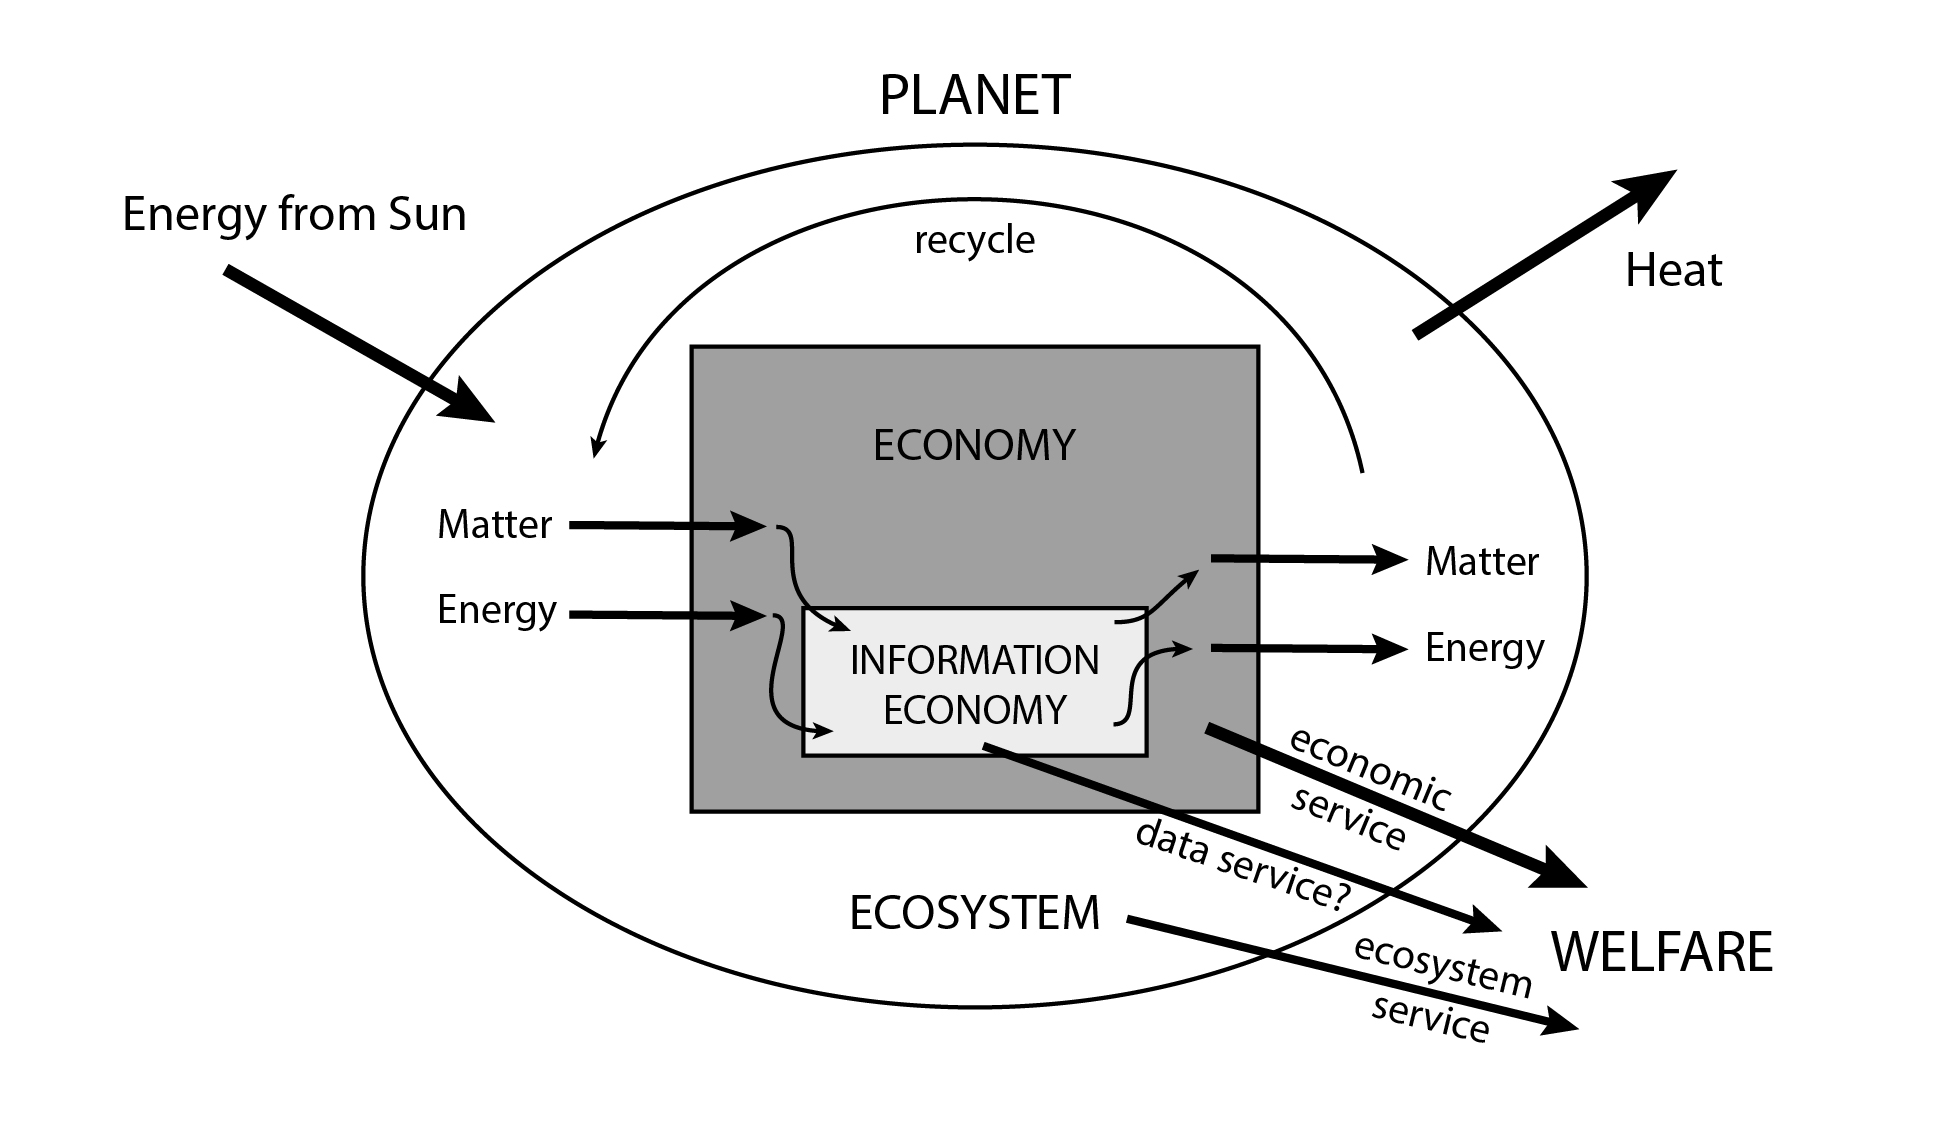
\includegraphics[width=5.5in]{figures/ecologicalecon}
  \caption{The information economy understood as a sector of the global economy which itself is a sub-system of the global ecosystem. This vision comes from ecological economics which is a project to turn the classical economic vision of the ecosystem as a part of the economy to the reverse, the economy is a part of the ecosystem. In a similar manner the information economy, data assemblages, or whatever name we choose, is also a part of the ecosystem an cannot be an ecosystem or ecology itself. Adapted from \citep[][p. 18]{daly_2004}}
\end{figure}

A question that arises from the figure. If the information economy is growing exponentially, where will it fit in the future (the outside circle cannot grow)? 10, 20, 50, 100 years? One of the biggest problems in libraries is physical space to store books. Will this be the same for digital objects? Some will argue that storage technology will continue to pack more information on to smaller and smaller devices. Indeed Kryder's law states that digital storage media costs drop exponentially (and have for the last thirty years). Is there a limit to this \citep[cf.][]{rosenthal_2012}?
 
How can we expand the current discussion of information ecology to make it more powerful for the future. We propose the following areas for improvement






